\section{Linear functionals on the tempered Paley--Wiener space}\label{sec:tempered-duality}
We now use the spectral coordinates of the preceding sections to describe invariant distributions. We distinguish the algebraic trace image from its smooth completion. All assertions about group distributions through a smooth block model use the corresponding topological trace theorem, not merely an algebraic parametrization.

\subsection{Sequence spaces and the constant mode}
Let $B_0=1$ and $B_n=z^n+z^{-n}$ for $n\ge1$. The variable $u=z+z^{-1}$ identifies the invariant Laurent polynomials with $\mathbb C[u]$. A smooth inversion-invariant circle function has a unique expansion $h=a_0+\sum_{n\ge1}a_nB_n$ with rapidly decreasing coefficients. Integration by parts in the angular variable gives rapid decay; conversely termwise differentiation of a rapidly decreasing series converges uniformly at every order. The constant coefficient $a_0$ is independent of the other coefficients and must not be omitted.

Let $s$ be the space of sequences with all seminorms $\sup_n(1+n)^k|a_n|$ finite, and let $\varphi$ be the finite sequences with the locally convex inductive-limit topology of their finite-dimensional coordinate spaces. The Fourier expansion identifies $C^\infty(S^1)^W$ topologically with $s$. The polynomial space is identified with $\varphi$. In the unramified block the smooth space is modeled by $s\oplus\mathbb C^2$, with coordinates $(h,d,b)$; $d$ is the quadratic constituent difference and $b$ is the Steinberg trace. The representation-theoretic identification of this model is discussed in Section~\ref{sec:pwcomparison}.

\begin{theorem}\label{thm:duality-moments}
A linear functional on $\varphi\oplus\mathbb C^2$ extends continuously to $s\oplus\mathbb C^2$ if and only if its moments $m_n=\lambda(B_n,0,0)$ satisfy $|m_n|\le C(1+n)^N$ for some $C,N$. The extension is unique, and its two exceptional coefficients are unrestricted.
\end{theorem}
\begin{proof}
Continuity bounds the functional by finitely many seminorms. Applying this bound to the coordinate vectors gives the necessary estimate. Conversely $\sum a_nm_n$ converges absolutely and is bounded by $C\sup_n(1+n)^{N+2}|a_n|\sum_n(1+n)^{-2}$. Add the two ordinary scalar functionals. Finite sequences are dense in $s$, proving uniqueness.
\end{proof}
For example, second angular differentiation at $z=1$ has moments $-2n^2$ for $n\ge1$ and zero constant moment. It is tempered in the spectral model. The generic ramified blocks use bilateral Laurent moments indexed by $\mathbb Z$; the proof is unchanged with $|n|$ in the weights. Ramified quadratic blocks use the same even sequence space and two independent constituent-difference coordinates.

\subsection{Reducibility as a split exact sequence}
Put $c=q+q^{-1}$. In the unramified algebraic block use ambient coordinates $(Q,x_+,x_-,t,b)$, where $t$ is the trivial trace. Define
\[
D(Q,x_+,x_-,t,b)=(x_++x_--Q(-2),\,t+b-Q(c)).
\]
The algebraic trace space is $\ker D$ by the good-functional theorem. The map has a continuous right inverse $(v,w)\mapsto(0,v,0,w,0)$ for the polynomial inductive-limit topology. Thus the sequence is split and its continuous dual is exact:
\[
0\longrightarrow(\mathbb C^2)'\xrightarrow{D'} A'
 \longrightarrow(\ker D)'\longrightarrow0,\qquad
 A=\mathbb C[u]\oplus\mathbb C^4.
\]
The image of $D'$ is generated by
$(-\operatorname{ev}_{-2},1,1,0,0)$ and
$(-\operatorname{ev}_c,0,0,1,1)$.
The same construction works in holomorphic spaces where both evaluations are continuous. In the tempered space the second relation must instead be removed along with the trivial coordinate: evaluation at $c$ is not defined continuously on smooth circle functions. There remains one constraint, $x_++x_-=h(-1)$, and an independent Steinberg coordinate. For a ramified quadratic block both sum constraints are circle evaluations and are continuous.

\begin{center}
\begin{tikzpicture}[>=stealth]
\node (e) at (0,1.5) {$E$};\node (a) at (3.5,1.5) {$A$};\node (c) at (7,1.5) {$\mathbb C^2$};
\node (ed) at (0,0) {$E'$};\node (ad) at (3.5,0) {$A'$};\node (cd) at (7,0) {$(\mathbb C^2)'$};
\draw[->] (e)--(a);\draw[->] (a)--node[above]{$D$}(c);
\draw[->] (cd)--node[below]{$D'$}(ad);\draw[->] (ad)--(ed);
\foreach \x/\y in {e/ed,a/ad,c/cd}{\draw[dashed,->] (\x)--(\y);}
\end{tikzpicture}
\end{center}
Solving the algebraic constraints gives $x_\pm=(Q(-2)\pm d)/2$ and $t=Q(c)-b$. Every spectral functional has a unique normal form
\[
\lambda(Q,d,b)=\sum_{n\ge0}a_nm_n+\alpha d+\beta b.
\]
For polynomials the sum is finite; in the smooth model it converges by Theorem~\ref{thm:duality-moments}. In particular the nonzero quadratic difference and Steinberg character both have zero Laurent moments. The exceptional coordinates are essential for uniqueness.

\subsection{Invariant distributions and global topology}
Let $H=C_c^\infty(G)$ and $S=\mathcal C(G)$. Conjugation invariance on $H$ is equivalent to vanishing on convolution commutators. Indeed a conjugation-invariant functional has equal values on $f*g$ and $g*f$ by integrating translates, and conversely a compact-open approximate identity expresses conjugation differences as commutators. For the latter, choose a compact-open subgroup fixing $f$ on both sides, write the conjugation difference as the commutator of a translated idempotent and a translated $f$, and use convolution associativity. The same equivalence holds for continuous functionals on $S$ by density of $H$ and continuity of multiplication and conjugation. Kazhdan density identifies the algebraic cocenter with the algebraic trace image. All linear forms on $H$ are continuous for its locally convex inductive limit of finite-dimensional support-and-level stages.

For Schwartz functions the required identity is $\ker T_t=\overline{[S,S]}$. Arthur's open trace theorem \cite[p.~174]{Ar94} identifies the quotient by its trace kernel topologically with the smooth trace image. Solleveld's survey on group algebras, Examples 5.10 and 5.12 and Theorem 5.14, is a source for the closed-commutator identification; its exact version and hypotheses must be reconciled with Arthur's topology. Until that verification is complete, the assertion that every invariant tempered distribution has the displayed normal form is conditional on this identification.

\begin{proposition}\label{prop:duality-global}
For a locally convex direct sum $E=\bigoplus_{\mathfrak s}E_{\mathfrak s}$, restriction identifies $E'$ with $\prod_{\mathfrak s}E_{\mathfrak s}'$.
\end{proposition}
\begin{proof}
A functional on the sum is continuous precisely when all restrictions are continuous, by the defining final locally convex topology. The inverse sends a family of functionals to the finite sum of their values on each test vector.
\end{proof}
\begin{center}
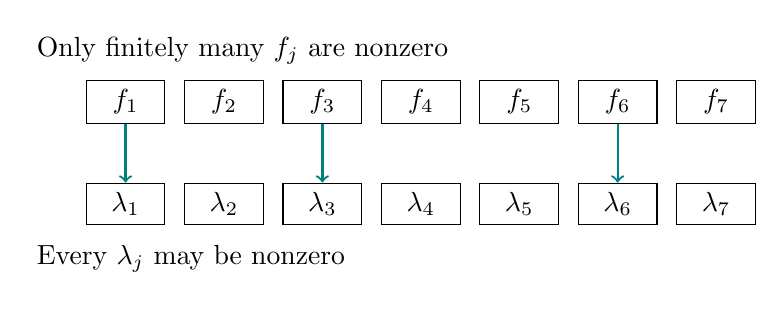
\begin{tikzpicture}
\foreach \n in {1,...,7}{
\node[draw,minimum width=1cm] (a\n) at (\n*1.25,1) {$f_{\n}$};
\node[draw,minimum width=1cm] (b\n) at (\n*1.25,-.3) {$\lambda_{\n}$};}
\foreach \n in {1,3,6}{\draw[teal,thick,->] (a\n)--(b\n);}
\node[anchor=west] at (0,1.65) {Only finitely many $f_j$ are nonzero};
\node[anchor=west] at (0,-1) {Every $\lambda_j$ may be nonzero};
\end{tikzpicture}
\end{center}
In the anticipated global Schwartz model the growth constants and exponents may depend on the block; a single uniform exponent is not required. To identify the topology, use the stages $S^{K_m\times K_m}$ for principal congruence subgroups $K_m$. Bernstein finiteness restricts each stage to finitely many blocks. The converse requires realization of the full smooth block trace image at sufficiently deep fixed level with continuous control of seminorms. Types and blockwise Morita equivalences are useful tools. See Solleveld, \emph{On completions of Hecke algebras}, arXiv:1612.01776, for a direction to investigate.

\subsection{Topologies on distribution spaces}
The weak dual topology is pointwise convergence on test vectors. The strong dual topology is uniform convergence on bounded subsets, and the compact-convergence topology is uniform convergence on compact subsets. On $\varphi'$ the strong dual topology is the ordinary product topology of all sequences, since bounded subsets of $\varphi$ lie in finite-dimensional stages. For $s'$ the standard strong dual sequence-space model is the inductive limit of weighted bounded sequence spaces with norms $\sup_n |m_n|/(1+n)^N$. In particular a family of tempered spectral functionals is equicontinuous exactly when it satisfies a common polynomial estimate. These facts distinguish individual growth from uniform estimates on families.

\section{Linear functionals on the admissible Paley--Wiener space}\label{sec:admissible-duality}
The admissible trace image is algebraic, but different completions of its polynomial coordinates provide intermediate dual spaces. We develop the Laurent criterion and then examine the action of the Bernstein center. The holomorphic models are spectral constructions; their identification with any independently defined notion of analytic distributions on $G$ is not assumed.

\subsection{The unified Laurent criterion}
For $r>1$ let $A_r=\{r^{-1}<|z|<r\}$. Append the same two exceptional scalar coordinates to each of the spaces below. Restriction gives dense continuous inclusions
\[
\mathbb C[z,z^{-1}]^W\ \longrightarrow\
\mathcal O(\mathbb C^\times)^W\ \longrightarrow\
\mathcal O(A_r)^W\ \longrightarrow\ C^\infty(S^1)^W.
\]
The holomorphic spaces have the compact-open topology. Density follows by Laurent truncation, or Fourier truncation on the circle. The continuous dual arrows reverse direction.
\begin{center}
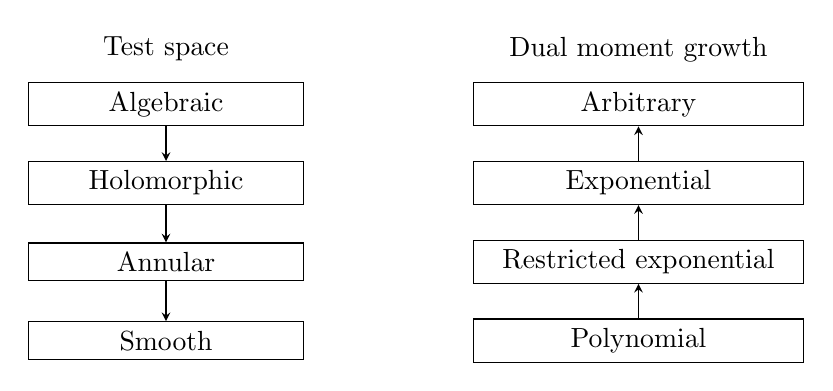
\begin{tikzpicture}[>=stealth]
\foreach \y/\a/\b in {3/Algebraic/Arbitrary,2/Holomorphic/Exponential,1/Annular/Restricted exponential,0/Smooth/Polynomial}{
\node[draw,minimum width=3.5cm] (l\y) at (0,\y) {\a};
\node[draw,minimum width=4.2cm] (r\y) at (6,\y) {\b};}
\foreach \i/\j in {3/2,2/1,1/0}{\draw[->] (l\i)--(l\j);\draw[->] (r\j)--(r\i);}
\node at (0,3.7) {Test space};\node at (6,3.7) {Dual moment growth};
\end{tikzpicture}
\end{center}
\begin{theorem}\label{thm:duality-holomorphic}
A linear functional with moments $m_n$ on the invariant Laurent polynomial space is continuous for the algebraic inductive limit without restriction. It extends continuously to $\mathcal O(\mathbb C^\times)^W$ precisely when $|m_n|\le CR^n$ for some $R>1$, and to $\mathcal O(A_r)^W$ precisely when such a bound holds with $1<R<r$. The smooth extension criterion is Theorem~\ref{thm:duality-moments}. Continuous extension to $C(S^1)^W$ holds precisely when the moments are the integrals of $B_n$ against a finite inversion-invariant complex measure.
\end{theorem}
\begin{proof}
For the holomorphic spaces put $p_R(h)=\sup_{R^{-1}\le|z|\le R}|h(z)|$, with $R<r$ in the annular case. A continuous functional is bounded by a single such seminorm up to a constant. Since $p_R(B_n)\le2R^n$, necessity follows. Conversely choose $R'>R$ within the allowed range. Cauchy's coefficient estimate yields $|a_n|\le p_{R'}(h)(R')^{-n}$. The defining moment sum converges absolutely and is bounded by a constant times $p_{R'}(h)\sum_{n\ge0}(R/R')^n$. Density proves uniqueness. For continuous circle functions, extend by composing with inversion averaging and apply the Riesz representation theorem; symmetrize the resulting finite complex measure. Conversely integration against such a measure is bounded for the uniform norm.
\end{proof}

\subsection{Growth radii and examples}
Define $\rho(\lambda)=\limsup_{n\to\infty}|m_n|^{1/n}$. The entire punctured-plane extension is equivalent to $\rho<\infty$, and the annular extension is equivalent to $\rho<r$. Tempered extension is strictly stronger than $\rho\le1$. For example $m_n=\exp(\sqrt n)$ has radius one and extends to every open annulus but fails every polynomial bound. The algebraic trace theorem realizes any moment sequence as an invariant distribution by pullback, including $m_n=n!$ which has no holomorphic extension.
\begin{center}\small
\begin{tabular}{lll}
\hline
Moments ($n\ge1$)& Radius & Tempered extension\\\hline
$1,\ n^3$ & $1$ & yes\\
$\exp(\sqrt n)$ & $1$ & no\\
$2^n$ & $2$ & no\\
$q^{sn}+q^{-sn}$ ($s>0$) & $q^s$ & no\\
$n!,\ \exp(n^2)$ & $\infty$ & no\\\hline
\end{tabular}
\end{center}
\begin{center}
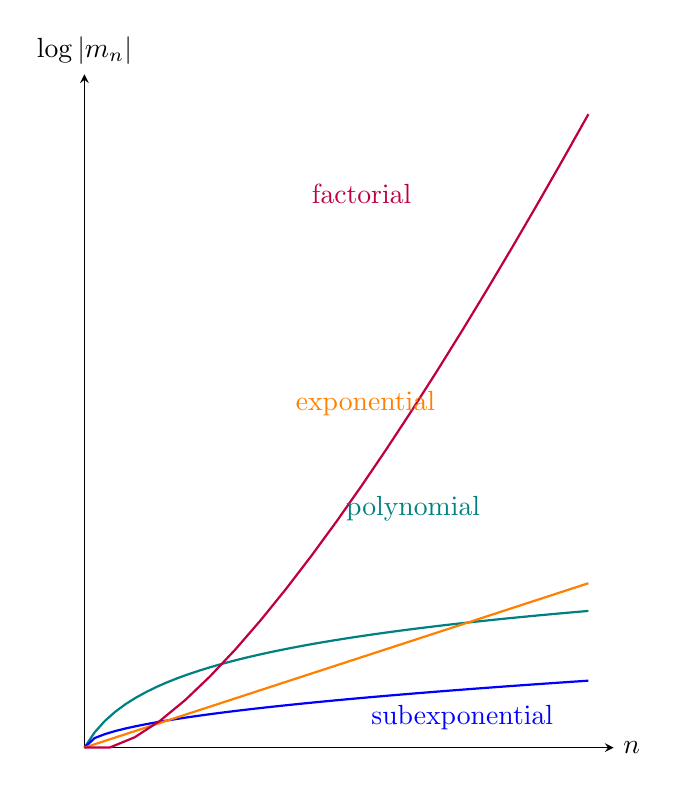
\begin{tikzpicture}[x=.32cm,y=.19cm,>=stealth]
\draw[->] (0,0)--(21,0) node[right]{$n$};
\draw[->] (0,0)--(0,45) node[above]{$\log |m_n|$};
\draw[teal,thick,domain=0:20,samples=50] plot (\x,{3*ln(\x+1)});
\draw[blue,thick,domain=0:20,samples=50] plot (\x,{sqrt(\x)});
\draw[orange,thick,domain=0:20] plot (\x,{\x*ln(3)/2});
\draw[purple,thick] plot coordinates {(0,0)(1,0)(2,.693)(3,1.792)(4,3.178)(5,4.787)(6,6.579)(7,8.525)(8,10.605)(9,12.802)(10,15.104)(11,17.502)(12,19.987)(13,22.552)(14,25.191)(15,27.899)(16,30.672)(17,33.505)(18,36.395)(19,39.340)(20,42.336)};
\node[teal,anchor=west] at (10,16) {polynomial};
\node[blue,anchor=west] at (11,2) {subexponential};
\node[orange,anchor=west] at (8,23) {exponential};
\node[purple] at (11,37) {factorial};
\end{tikzpicture}
\end{center}
The principal-series trace is evaluation of $Q$ at $z+z^{-1}$. The quadratic characters are $(Q(-2)\pm d)/2$, the Steinberg character is $b$, and the trivial character is $Q(c)-b$. Complementary-series evaluation at $z=q^{-s}$ has moments $q^{sn}+q^{-sn}$ and $\rho=q^s$, so $s=\log\rho/\log q$. Trivial evaluation has radius $q$ and extends to $A_r$ exactly for $r>q$. Pure exceptional functionals have all moments zero, including the constant moment. Their growth radius is zero regardless of their nonzero exceptional coefficients.

\subsection{The Bernstein center and a discrete recurrence}
The unramified Bernstein center $\mathbb C[u]$ acts by
\[
p\cdot(Q,d,b)=(pQ,p(-2)d,p(c)b).
\]
On the dual use $(p\lambda)(f)=\lambda(pf)$. For $n\ge2$, $uB_n=B_{n+1}+B_{n-1}$, while $uB_0=B_1$ and $uB_1=B_2+2B_0$.
\begin{theorem}\label{thm:duality-eigen}
If $u\lambda=\mu\lambda$, then
\[
m_1=\mu m_0,\quad m_2+2m_0=\mu m_1,\quad
m_{n+1}+m_{n-1}=\mu m_n\quad(n\ge2).
\]
Writing $\mu=z_0+z_0^{-1}$, the unique solution is $m_n=m_0(z_0^n+z_0^{-n})$ for $n\ge1$. The exceptional coefficients satisfy $(-2-\mu)\alpha=(c-\mu)\beta=0$.
\end{theorem}
\begin{proof}
Apply the eigen-equation to the polynomial basis and to the two exceptional coordinate vectors. The displayed evaluation sequence satisfies all initial conditions and the recurrence, which determines it uniquely.
\end{proof}
Thus the central eigenspace has dimension one except at $-2,c$, where it has dimension two. This recovers the exceptional support fibers through duality.
\begin{center}
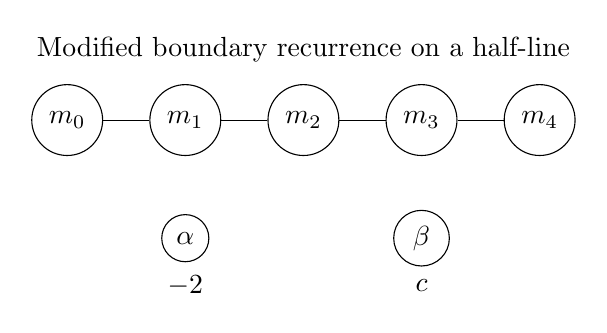
\begin{tikzpicture}
\foreach \n in {0,...,4}{\node[circle,draw,minimum size=9mm] (v\n) at (1.5*\n,0) {$m_{\n}$};}
\foreach \n/\m in {0/1,1/2,2/3,3/4}{\draw (v\n)--(v\m);}
\node at (3,.9) {Modified boundary recurrence on a half-line};
\node[circle,draw] at (1.5,-1.5) {$\alpha$};
\node[circle,draw] at (4.5,-1.5) {$\beta$};
\node at (1.5,-2.1) {$-2$};\node at (4.5,-2.1) {$c$};
\end{tikzpicture}
\end{center}
This is a tridiagonal sequence model, not the literal Bruhat--Tits adjacency operator. Comparison with the radial Satake operator is a possible further direction.

\subsection{Generalized central eigendistributions}
\begin{theorem}\label{thm:duality-jets}
For $m\ge1$, the space of functionals satisfying $(u-\mu)^m\lambda=0$ has dimension
$m+\mathbf1_{\{\mu=-2\}}+\mathbf1_{\{\mu=c\}}$. Its polynomial part consists of the evaluation jets $Q\mapsto Q^{(j)}(\mu)$ for $0\le j<m$.
\end{theorem}
\begin{proof}
The polynomial functional factors through $\mathbb C[u]/(u-\mu)^m$. Taylor expansion gives the stated basis of the dual of this quotient. Each exceptional summand is one-dimensional and is annihilated by $(u-\mu)^m$ exactly at its central character.
\end{proof}
For $\mu\in[-2,2]$, Markov's inequality for polynomial derivatives on a compact interval gives polynomial growth of the jet moments, since $B_n=2T_n(u/2)$ has degree $n$ and supremum two there. In particular $B_n'(2)=n^2$. For $\mu\notin[-2,2]$, choose the root $z_0$ of $z+z^{-1}=\mu$ with $|z_0|>1$. It varies holomorphically locally with $\mu$ and has nonzero logarithmic derivative. A nonzero linear combination of jets of highest order $j$ has leading moment $z_0^n$ times a polynomial of degree $j$ with nonzero leading coefficient, plus an exponentially decreasing term times a polynomial. It cannot be polynomially bounded. At $\mu=c$ the independent Steinberg functional remains tempered even though the polynomial jets do not. Thus the central character alone does not decide temperedness.

\subsection{Generating functions and central finiteness}
Define the formal series $F_\lambda(w)=\sum_{n\ge0}m_nw^n$. Its analytic radius is $1/\rho$ by Cauchy--Hadamard, with the usual zero and infinity conventions. For evaluation at $\mu$,
\[
F_\lambda(w)=\frac{1-w^2}{1-\mu w+w^2}.
\]
Evaluation at $2$ gives $(1+w)/(1-w)$ and evaluation at $-2$ gives $(1-w)/(1+w)$. Jets give derivatives of the rational expression. Pure exceptional functionals give zero.
\begin{proposition}\label{prop:duality-rational}
Central finiteness (finite-dimensional span of $\mathbb C[u]\lambda$) implies rationality of $F_\lambda$, but the converse is false in general.
\end{proposition}
\begin{proof}
A finite-dimensional central module is annihilated by a nonzero polynomial. Factoring that polynomial and using the Chinese remainder theorem expresses the polynomial functional as a finite sum of jets. Their generating functions are rational. For the converse counterexample, take $m_0=0$, $m_1=1$, and $m_n=0$ for $n\ge2$. Then $F_\lambda(w)=w$ is rational. The functional is proportional to extraction of the coefficient of $z$ from an invariant Laurent polynomial. No nonzero $p(u)$ annihilates it: the bilinear constant-coefficient pairing on symmetric Laurent polynomials is nondegenerate, since the basis $B_n$ is orthogonal with nonzero diagonal values. The functional equals constant-coefficient pairing with $B_1/2$, so annihilation would force $p(u)B_1=0$, impossible in the Laurent polynomial domain.
\end{proof}
The exact replacement criterion is rationality of the monomial moment series $M_\lambda(t)=\sum_{n\ge0}\lambda(u^n,0,0)t^n$. An eventual recurrence of its coefficients produces an annihilating polynomial after multiplying by a sufficiently large power of $u$; conversely an annihilating polynomial yields a recurrence. Exceptional summands can be killed by multiplying by $(u+2)(u-c)$. The formal identity
\[
F_\lambda(w)=\frac{1-w^2}{1+w^2}
M_\lambda\left(\frac{w}{1+w^2}\right)
\]
explains why rationality of $M_\lambda$ implies rationality of $F_\lambda$ but not conversely. The distinction matters for any comparison with quasi-finiteness in Section~\ref{sec:descent}.

\subsection{Exceptional modes and further questions}
The subspace with zero polynomial moments in the chosen unramified splitting is spanned by the quadratic character difference and the Steinberg character. In ramified quadratic blocks it is spanned by the two constituent differences. All are tempered. The subspace depends on the splitting: with the algebraic difference coordinate of Subsection~\ref{subsec:pw-coordinates} in place of the Steinberg trace it is a different subspace. Theorems~\ref{thm:twosplit} and~\ref{thm:exact} give the intrinsic description by weak constant terms and compare the two splittings; literal elliptic support is a different notion. The remaining tasks are to identify the global smooth topology and its cocenter, compare analytic spectral functionals with group-side decay or analyticity, and compare central finiteness with the original quasi-finiteness definition. None of these identifications is inferred solely from the elementary moment calculations.
